% Folger
\newcommand{\summ}{\cmc{Sum}{<Uttrykk>, <Variabel>, <Start>, <Slutt>} Finner summen av en rekke med en løpende variabel på et intervall.}
\newcommand{\rsumm}{\rgg{\summ}}
\newcommand{\rsumme}{\eks{
		Finn summen av den uendelige rekka ..
		\[ 1+ \frac{1}{5} + \frac{1}{25} +...  \]	
		
		\sv
		Dette er en geometrisk rekke med $ {k=\frac{1}{5}} $ og eksplisitt formel gitt som:
		\[ a_n = \frac{1}{5^{(n-1)}} \] 	
		hvor $ {n\in[1, 2, ...]} $. \vsk
		
		I CAS skriver vi da ($ \infty $-tegnet finner du ved å trykke på $ \alpha$-tegnet oppe i høyre hjørne):
		\begin{center}
			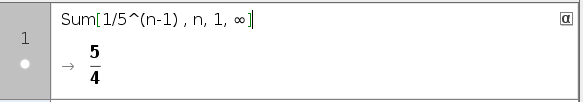
\includegraphics[scale=0.5]{fig/rek}
		\end{center}
		
	}}
% Trigonometri
\newcommand\los{
	\cmc{Løs}{<Likning med x>}
	Løser en likning med $ x $ som ukjent.	
}
\newcommand{\rtrilig}{\rgg{\los}}		
\newcommand{\rtrilige}{\eks{
		\vs
		\begin{figure}
			\centering
			\includegraphics[scale=0.5]{\scr{trilig}}
		\end{figure}	
		I \textit{Før Kalkulus; Teoridel}  brukes $ {n\in \mathbb{Z}} $ som heltallsvariabel, GeoGebra bruker en indeksert $ k $ (her $ {k_1 \in \mathbb{Z}})$. \vsk
		
		\textsl{Merk}: Du kan også løse ligningen $ {\sin(3x)=1 }$ ved å skrive den inn i en CAS-celle og deretter trykke på \texttt{Løs}.
	}}

\newcommand\trikomb{
	\cm{TrigKombiner}{<Funksjon>, sin(x)}
	Skriver om en funksjon på formen $ {a\sin (kx) + b\cos (kx) }$ til et kombinert uttrykk på formen $ r\sin (kx+c) $.	
}
\newcommand\regsin{
	\cm{RegSin}{<Liste>}
	Bruker regresjon med en sinusfunksjon for å tilpasse punkt gitt i en liste.	
}

\newcommand{\rtrikomb}{\rgg{\trikomb}}
\newcommand{\rtrikombe}{\eks{
		\begin{figure}
			\centering
			\includegraphics[scale=0.5]{\scr{trikomb}}
		\end{figure}
	}}
\newcommand{\rregsin}{\rgg{\regsin\vspace{0pt}}}

\newcommand{\rregsine}{\eks{
		Gitt tabellen \vs
		\begin{center}
			\begin{tabular}{|c | c|}
				\hline
				$ x $ & $ f(x) $ \\
				\hline
				1 & -2.12 \\
				\hline
				2 & -2.73 \\
				\hline
				3 & -0.62 \\
				\hline
				4 & 2.37 \\
				\hline
				5 & 2.88\\	
				\hline	
			\end{tabular}
		\end{center}
		Bruk regresjon for å finne en tilnærming til $ f(x) $ uttrykt som en sinusfunksjon. \vsk
		
		\sv	
		Vi velger
		{\tt Vis $ \blacktriangleright $ Regneark} og skriver inn tabellen. Vi markerer så begge kolonner, høyreklikker innenfor markeringsfeltet og velger \\{\tt Lag $ \blacktriangleright $ Liste med punkt}:
		\begin{figure}
			\centering
			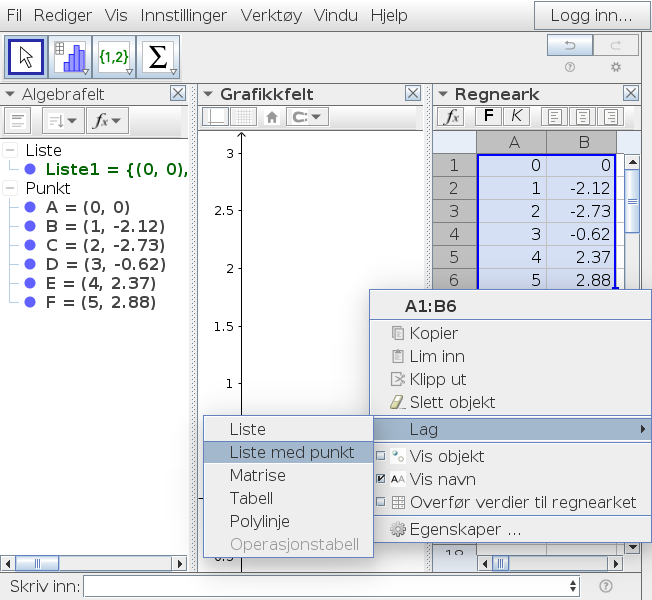
\includegraphics[scale=0.3]{fig/reg}
		\end{figure} 
		Om vi ønsker at alle punktene skal vises i grafikkfeltet, høyreklikker vi på grafikken og velger {\tt Vis alle objekt}. Deretter skriver vi {\tt RegSin[Liste1]} i kommandolinjen, og får funksjonen {\tt f(x)} i algebrafeltet og grafen til \texttt{f} i grafikkfeltet. Denne funksjonen er en tilnærming til $ f(x) $ gitt i oppgaven.
		\begin{figure}
			\centering
			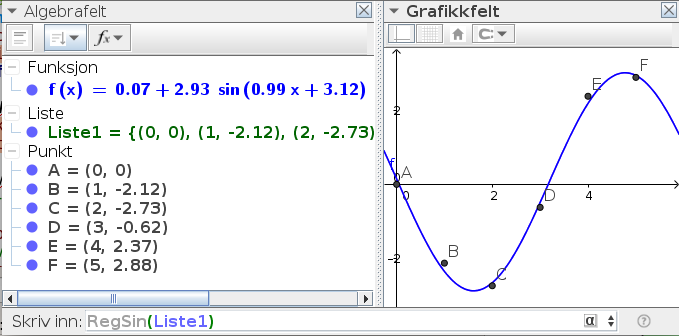
\includegraphics[scale=0.3]{fig/reg2}
		\end{figure} 
	}}
%Vektorer
\newcommand{\punkt}{
\cm{Punkt}{<Liste>} Lager et punkt med koordinater gitt som liste. 

\merk For å lage punktet $ (x, y, z) $ kan man liksågodt skrive \texttt{(x,y,z)} i inntastingsfeltet. Skriver man \texttt{(x,y,z)} i CAS lager man vektoren $ [x, y, z] $.
}
\newcommand{\vektor}{
\cm{Vektor}{<Punkt>} Lager vektoren fra origo til et gitt punkt. 

\merk I CAS kan man lage vektoren $ {[x, y, z]} $ ved å skrive \texttt{(x,y,z)}, dette anbefales.
}
\begin{comment}
	\newcommand{\deter}{
	\cm{Determinant[ <Matrise> ]} Finner determinanten til en matrise.	
	}
	\newcommand{\rdeter}{\rgg{\deter}}
	\newcommand{\rdetere}{\eks{
	Regn ut:
	\[ \left|\begin{matrix}
	1 & -2 & 2 \\
	2 & 2 & -3 \\
	4 & -1 & 2
	\end{matrix}\right| \]
	\sv
	\vs
	\vs
	\begin{figure}
	\centering
	\includegraphics[scale=0.5]{\scr{det}}
	\end{figure}
	}}
\end{comment}
% Rom
\newcommand\skalar{
	\cm{Skalarprodukt}{<Vektor>, <Vektor>} 
	Finner skalarproduktet av to vektorer. 
	
	\merk For to vektorer $u$ og $v$ kan man like gjerne skrive \texttt{u*v}.	
}
\newcommand{\rskalar}{\rgg{\skalar}}
\newcommand\vekpro{
	\cmc{Vektorprodukt}{<Vektor>, <Vektor>}
	Finner vektorproduktet av to vektorer. (Merk: For to vektorer $u$ og $v$ kan man like gjerne skrive \texttt{u}$ \otimes $\texttt{v}. Hurtigtast for $ \otimes $ er \texttt{alt+shift+8}).		
}
\newcommand{\rvekpro}{\rgg{\vekpro}}
\newcommand\pyr{
	\cm{Pyramide}{<Punkt>, <Punkt>, ...}
	Framstiller en pyramide i Grafikkfelt 3D. {\tt Pyramide[A,B,C,D]} lager en pyramide med grunnflate ${ A, B, C} $ og toppunkt $ D $, mens {\tt Pyramide[A,B,C,D, E]} har grunnflate ${ A, B, C, D }$ og toppunkt $ E $. Under kategorien \textsl{Pyramide} i algebrafaltet finner man en konstant som oppgir volumet til pyramiden.}
\newcommand{\rpyr}{\rgg{\pyr}}
\newcommand\pris{
	\cm{Prisme}{<Punkt>, <Punkt>, ...}
	Framstiller en prisme i Grafikkfelt 3D. {\tt Prisme[A,B,C,D]} lager en prisme med grunnflate $ ABC $ og tak $ DEF $, {\tt Prisme[A,B,C,D,E]} har grunnflate $ ABCD $ og tak $ EFG $. $ F, G$ og eventelt $ E $ blir konstruert av GeoGebra slik at hver sideflate er et parallellogram. Under kategorien \textsl{Prisme} i algebrafaltet finner man en konstant som oppgir volumet til pyramiden.
}
\newcommand{\rpris}{\rgg{\pris\vs}}
\newcommand\kurve{
	\cm{Kurve}{<Uttrykk>, <Uttrykk>, <Uttrykk>, <Parametervariabel>, <Start>, <Slutt>}
	Viser parameteriseringen av en kurve i Grafikkfelt 3D på et gitt intervall. Uttrykkene er henholdsvis uttrykkene for $ {x, y} $ og $ z $-koordinatene, bestemt av en gitt parametervariabel.
	
	\merk Med mindre et bestemt intervall av kurven er ønsket, er det bedre å skrive parameteriseringen direkte inn i inntastingsfeltet som \texttt{A+t*u}, hvor $ A $ er et punkt på linja og $ u$ er en retningsvektor.
}	
\newcommand{\rkurve}{\rgg{\kurve}}
\newcommand\kuler{
	\cm{Kule}{<Punkt>, <Radius>}
	Viser en kule i Grafikkfelt 3D med sentrum i et gitt punkt og med en gitt radius.		
}
\newcommand{\rkuler}{\rgg{\kuler}}
\newcommand{\rkulere}{\eks{
		En linje $ l $ med parameteriseringen
		\[l: \left\lbrace{
			\begin{array}{lll}
			x=-3 -2t   \\
			y= 1 +t    \\
			z= 4 + 2t 
			\end{array}
		}\right. \]	
		skjærer en kule med med sentrum i $ {(-1, 2, 6) }$ og radius lik 3. \vsk
		
		\textbf{a)} Tegn kula og linja.
		
		\textbf{b)} Finn skjæringspunktet mellom kula og linja. \vsk
		
		\sv
		Vi skal her se på to løsningsmetoder. Den første metoden er helt klart den raskeste, men den andre metoden er tatt med for å illustrere bruken av \texttt{Kurve}-kommandoen, i tillegg til å presentere en metode som vil sikre oss eksaktverdier.\vsk
		
		\textit{Løsningsmetode 1}\vsk
		
		\textbf{a)} 
		\begin{figure}
			\centering
			\includegraphics[scale=0.4]{\scr{skjlinkul}}
		\end{figure}
		Vi starter med å tegne kula. I inntastingsfeltet skriver vi \texttt{Kule[(-1, 2, 6), 3]} og får kula $ a $ i algebrafelt og grafikkfelt 3D. For å tegne linja skriver vi
		\texttt{(-3, 1, 4)+t*(2,1,2)} i inntastingsfeltet, resultatet er kurven $ f $.\vsk
		
		\textbf{b)} 
		\begin{figure}
			\centering
			\includegraphics[scale=0.4]{\scr{skjlinkulb}}
		\end{figure}
		I inntastingsfeltet skriver vi \texttt{Skjæring[a, f]} og får de to punktene $ A $ og $ B $. (Merk: Hadde vi tegnet linja ved hjelp av \texttt{Kurve}-kommandoen, ville ikke dette funket. \texttt{Skjæring} er ikke kompatibel med \texttt{Kurve}, og i dette tilfellet heller ikke med CAS)\vsk
		
	\textit{Løsningsmetode 2}\vsk
	
	\textbf{a)} 
	\begin{figure}
		\centering
		\includegraphics[scale=0.4]{\scr{skjlinkul2}}
	\end{figure}
	For å tegne linja skriver vi her
	\texttt{Kurve[-3 + 2t, 1 + t, 4 + 2t, t, -10, 10]} i inntastingsfeltet. At ${ t\in[-10, 10] }$ velger vi ut ifra inspeksjon i grafikkfelt 3D, det gjelder å velge et intervall som viser begge skjæringspunktene mellom kula og linja (man kan velge $ {t\in[-\infty, \infty] }$, men da blir ikke kurven vist grafikkfeltet). Resultatet er kurven $ b $.\vsk
	
	\textbf{b)} 
	\begin{figure}
		\centering
		\includegraphics[scale=0.5]{\scr{skjlinkulb2}}
	\end{figure}
	I CAS-celle 1 lager vi oss en ny funksjon $ {k(x, y, z) }$ med et uttrykk tilsvarende venstresiden til kuleligningen. For at linja skal skjære kula, må parameteriseringen til linja oppfylle kuleligningen. I CAS-celle 2 setter vi derfor uttrykkene for $ x, y $ og $ z $ fra parameteriseringen inn i $ k $, og krever at dette uttrykket skal bli lik $ 3^2 $. Vi trykker så på \texttt{Løs}-knappen og får to svar for $ t $. I CAS-celle 3 og 4 finner vi punktene for dissse valgene av $ t $.		
	}}

\newcommand\plan{
	\cm{Plan}{<Punkt>, <Punkt>, <Punkt>}
	Viser et plan i Grafikkfelt 3D, utspent av to av vektorene mellom tre gitte punkt.
}
\newcommand{\rplan}{\rgg{\plan}}
\newcommand{\hoyde}{\cm{Høyde}{<Objekt>}Gir avstanden fra toppunkt til grunnflate i et objekt. 
	
\merk Avstanden har retning, og derfor kan den noen ganger være negativ. Tallverdien er den geometriske høyden.}
\newcommand{\rh}{\rgg{\hoyde}}
\newcommand{\rhe}{\eks{
		Finn volumet og høyden til tetraetedet med grunnflate gitt ved punktene $ {A=(3, 2, 1)} $, $ {B=(6, 2, 1)} $, $ {C=(3, 6, 1)} $ og toppunkt ${ D=(5, 4, 3)} $.\vsk
		
		\sv
		Vi skriver inn punktene og bruker deretter kommandoen \texttt{Pyramide[A, B, C, D]} for å lage tetraedet $ a $. Algebrafeltet gir oss da at volumet til $ a $ er 4. I CAS-celle 1 finner vi høyden, som er 2.
		\begin{figure}
			\centering
			\includegraphics[scale=0.35]{\scr{pyr}}
		\end{figure}	
	}}
\newcommand{\linje}{\cm{Linje}{<Punkt>, <Punkt>} Gir uttrykket til en linje mellom to punkt. Hvis punktene har tre koordinater besår uttrykket av et punkt på linja og en fri variabel $ \lambda $ mulitplisert med en retningsvektor.}
\newcommand{\rlinje}{\rgg{\linje}}
\newcommand{\rlinjee}{\eks{Finn parameteriseringen til linja som går mellom punktet $ {(-2, 1, 3)}$ og ${ (-5, -1, 4)} $. \vsk
		
		\sv
		Vi skriver punktene i inntastingsfeltet og får punktene $ A $ og $ B $. Etterpå skriver vi \texttt{Linje[A, B]} og får da linjen $ f $.
		\begin{figure}
			\centering
			\includegraphics[scale=0.4]{\scr{linje}}
		\end{figure}
		Av dette finner vi at parameteriseringen til linja er gitt som:
		\[f: \left\lbrace{
			\begin{array}{lll}
			x=-2 -3t   \\
			y= 1 -2t    \\
			z= 3 + t 
			\end{array}
		}\right. \]	
	}}
\newcommand{\avst}{\cm{Avstand}{<Punkt>, <Objekt>}
	Gir avstanden fra et punkt til et objekt.}

\newcommand{\vink}{\cm{Vinkel}{<Vektor>, <Vektor>}
	Gir vinkelen mellom to vektorer. Kan også brukes for vinkel mellom plan/linjer, plan/plan og linje/linje}

% Derivasjon og funksjondrøfting
\newcommand{\der}{
	\cm{Deriverte}{<Funksjon>}	
	Gir den deriverte av en funksjon.
	
	\merk For en definert funksjon $ f(x) $, kan man like gjerne skrive \texttt{f'(x)}.
}
\newcommand{\deru}{\rgg{\der}}

\newcommand{\absmaks}{\cm{Maks}{<Funksjon>, <Start x-verdi>, <Slutt x-verdi>} Finner absolutt maksimum og maskimalpunkt for en funksjon $ f $ på et gitt intervall.}

\newcommand{\absmin}{\cm{Min}{<Funksjon>, <Start x-verdi>, <Slutt x-verdi>} Finner absolutt minimum og minimumspunkt for en funksjon $ f $ på et gitt intervall.}

\newcommand{\ekstpkt}{\cm{Ekstremalpunkt}{<Funksjon>, <Start>, <Slutt> } Finner alle lokale ekstremalpunkt og ekstremalverdier for en funksjon $ f $ på et gitt intervall.}

\newcommand{\vend}{
	\cm{Vendepunkt}{<Polynom>}
	Finner vendepunktene til et polynom.	
}
\newcommand{\rvend}{\rgg{\vend}}
% Integral

\newcommand\intu{
	\cm{Integral}{<Funksjon>}
	Gir uttrykket til det ubestemte integralet av en funksjon. (Merk: Hvis kommandoen skrives i inntastingsfeltet, blir konstantleddet utelatt).	
}
\newcommand{\rintu}{\rgg{\intu}}
\newcommand{\rintue}{\eks{
		\vs
		\begin{figure}
			\centering
			\includegraphics[scale=0.5]{\scr{int}}
		\end{figure}	
		$ c_1 $ er en vilkårlig konstant.
	}}
	\newcommand\intb{
		\cm{Integral}{<Funksjon>, <Start>, <Slutt>}
		Gir det bestemte integralet av en funksjon på et intervall.	
	}
	\newcommand{\rintb}{\rgg{\intb}}
	\newcommand{\rintbe}{\eks[1]{
			\vs
			\begin{figure}
				\centering
				\includegraphics[scale=0.5]{\scr{intb}}
			\end{figure}	
		}}
		\newcommand{\omdree}{\eks[2]{
				Finn volumet av omdreiningslegemet til $ {f(x)=x^2 }$ på intervallet $ {[0, 1]} $. \vsk
				
				\sv
				\begin{figure}
					\centering
					\includegraphics[scale=0.5]{\scr{omdr}}
				\end{figure}	
				I celle 1 definerer vi $ f(x) $. Volumet er gitt som ${\pi \int\limits_0^1 (f(x))^2\,dx} $, som vi finner i celle 2.		
			}}
% Diffligninger
\newcommand\dif{
	\cmc{LøsODE}{<Likning>}
	Finner generell løsning av en gitt differensialligning av første eller andre orden.
}
\newcommand{\rdif}{\rgg{\dif}}
\newcommand{\rdife}{\eks[1]{
		Løs ligningen:
		\[ y'+2y=2 \]
		\sv \vs \vs
		\begin{figure}
			\centering
			\includegraphics[scale=0.5]{\scr{dif1}}
		\end{figure}	
		$ c_1 $ er en vilkårlig konstant.
	}}
	\newcommand{\rdifeto}{\eks[2]{
			Løs ligningen:
			\[ y'+5y^2=0 \]
			\sv \vs \vs
			\begin{figure}
				\centering
				\includegraphics[scale=0.5]{\scr{dif2}}
			\end{figure}	
			$ c_1 $ er en vilkårlig konstant.
		}}
		\newcommand{\rdifetre}{\eks[3]{
				Løs ligningen:
				\[ y''+y'-6y=0 \]
				\sv \vs \vs
				\begin{figure}
					\centering
					\includegraphics[scale=0.5]{\scr{dif4}}
				\end{figure}	
				$ c_1 $ og $ c_2 $ er en vilkårlige konstanter.
			}}
			\newcommand\diff{
				\cmc{LøsODE}{<Likning>, <Punkt på f>, <Punkt på f'>}
				Finner løsningen av en gitt differensialligning av første eller andre orden, for randverdier gitt som punkter.
			}
			\newcommand{\rdiff}{\rgg{\diff}}
\newcommand{\rdiffe}{\eks[1]{
		Finn løsningnen av ligningen
		\[ y'-3y = 0 \]
		med randbetingelsen ${ y(0)=5} $.\vsk
		
		\sv 
		Randbetingelsen gir oss punktet $ {(x_0, y(x_0))=(0, 5)} $:
		\begin{figure}
			\centering
			\includegraphics[scale=0.5]{\scr{dif5}}
		\end{figure}	
	}}
		\newcommand\retn{
			\cmk{Retningsdiagram}{f(x,y)}
			Lager et retningsdiagram for en differensialligning hvor $ f(x,y)=y' $.	
		}
		\newcommand{\rretn}{\rgg{\retn}}

% Andre
\newcommand{\funk}{\cm{Funksjon}{<Funksjon>, <Start>, <Slutt>}
	Tegner en funksjon på et gitt intervall.}